\documentclass[aps,prb,twocolumn,superscriptaddress,floatfix,longbibliography]{revtex4-2}

\usepackage[utf8]{inputenc}
\usepackage[spanish]{babel}
\usepackage{graphicx}
\usepackage{amsmath}
\usepackage{subcaption}
\usepackage{wrapfig} 
\usepackage[export]{adjustbox}

\usepackage{amsmath,amssymb} % math symbols
\usepackage{bm} % bold math font
\usepackage{graphicx} % for figures
\usepackage{comment} % allows block comments
\usepackage{textcomp} % This package is just to give the text quote '
\usepackage{listings} %para agregar código

%\usepackage{ulem} % allows strikeout text, e.g. \sout{text}

\usepackage[spanish]{babel}

\usepackage{enumitem}
\setlist{noitemsep,leftmargin=*,topsep=0pt,parsep=0pt}

\usepackage{xcolor} % \textcolor{red}{text} will be red for notes
\definecolor{lightgray}{gray}{0.6}
\definecolor{medgray}{gray}{0.4}

\usepackage{hyperref}
\hypersetup{
colorlinks=true,
urlcolor= blue,
citecolor=blue,
linkcolor= blue,
bookmarks=true,
bookmarksopen=false,
}

% Code to add paragraph numbers and titles
\newif\ifptitle
\newif\ifpnumber
\newcounter{para}
\newcommand\ptitle[1]{\par\refstepcounter{para}
{\ifpnumber{\noindent\textcolor{lightgray}{\textbf{\thepara}}\indent}\fi}
{\ifptitle{\textbf{[{#1}]}}\fi}}
%\ptitletrue  % comment this line to hide paragraph titles
%\pnumbertrue  % comment this line to hide paragraph numbers

% minimum font size for figures
\newcommand{\minfont}{6}

% Uncomment this line if you prefer your vectors to appear as bold letters.
% By default they will appear with arrows over them.
% \renewcommand{\vec}[1]{\bm{#1}}

%Cambiar Cuadros por Tablas y lista de...
%\renewcommand{\listtablename}{Índice de tablas}
\renewcommand{\tablename}{Tabla}
\renewcommand{\date}{Fecha}

% \graphicspath{ {C:/Users/lupam/Mi unidad/Pablo Chehade/Instituto Balseiro (IB)/Laboratorio Avanzado/Informe/V5/Figures} } %Para importar imagenes desde una carpeta


\lstset{
  basicstyle=\ttfamily\small,
  breaklines=true,
  frame=single,
  numbers=left,
  numberstyle=\tiny,
  keywordstyle=\color{blue},
  commentstyle=\color{green},
  stringstyle=\color{red},
} %Configuración para el bloque de código


\usepackage[bottom]{footmisc} %para que las notas al pie aparezcan en la misma página



\begin{comment}

%Comandos de interes:

* Para ordenar el documento:
\section{Introducción}
\section{\label{sec:Formatting}Formatting} %label para luego hacer referencia a esa sección

\ptitle{Start writing while you experiment} %pone nombre y título al documento dependiendo de si en el header están los comandos \ptitletrue y \pnumbertrue

* Ecuaciones:
\begin{equation}
a^2+b^2=c^2 \,.
\label{eqn:Pythagoras}
\end{equation}

* Conjunto de ecuaciones:
\begin{eqnarray}
\label{eqn:diagonal}
\nonumber d & = & \sqrt{a^2 + b^2 + c^2} \\
& = & \sqrt{3^2+4^2+12^2} = 13
\end{eqnarray}

* Para hacer items / enumerar:
\begin{enumerate}
  \item
\end{enumerate}

\begin{itemize}
  \item
\end{itemize}

* Figuras:
\begin{figure}[h]
    \includegraphics[clip=true,width=\columnwidth]{pixel-compare}
    \caption{}
     \label{fig:pixels}
\end{figure}

* Conjunto de figuras:
(no recuerdo)


* Para hacer referencias a fórmulas, tablas, secciones, ... dentro del documento:
\ref{tab:spacing}

* Para citar
Elementos de .bib
\cite{WhitesidesAdvMat2004}
url
\url{http://www.mendeley.com/}\\

* Agradecimientos:
\begin{acknowledgments}
We acknowledge advice from Jessie Zhang and Harry Pirie to produce Fig.\ \ref{fig:pixels}.
\end{acknowledgments}

* Apéndice:
\appendix
\section{\label{app:Mendeley}Mendeley}

* Bibliografía:
\bibliography{Hoffman-example-paper}

\end{comment}



\begin{document}

% Allows to rewrite the same title in the supplement
\newcommand{\mytitle}{Aprendizaje supervisado en redes multicapa}

\title{\mytitle}

\author{Pablo Chehade \\
    \small \textit{pablo.chehade@ib.edu.ar} \\
    \small \textit{Redes Neuronales, Instituto Balseiro, CNEA-UNCuyo, Bariloche, Argentina, 2023} \\}
    
\maketitle

\section*{Ejercicio 1}

Se implementaron dos arquitecturas para el aprendizaje de la regla XOR, las cuales se ilustran en la figura \ref{fig:ej1_arquitectura}, considerando, en cada caso, una entrada adicional para simular el bias.

\begin{figure}[h]
    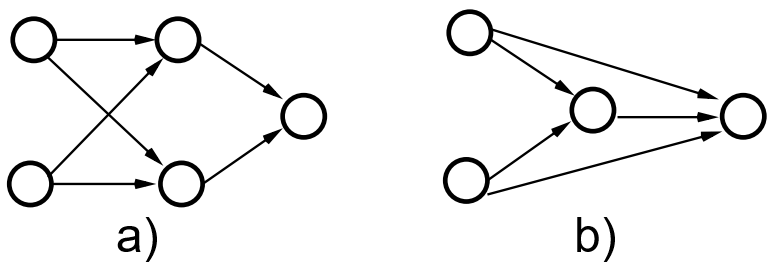
\includegraphics[clip=true,width=\columnwidth]{ej1_arquitectura.png}
    \caption{Arquitecturas utilizadas para el aprendizaje de la regla XOR, denominadas como arquitecturas a) A y b) B.}
     \label{fig:ej1_arquitectura}
\end{figure}

\begin{figure}[h]
    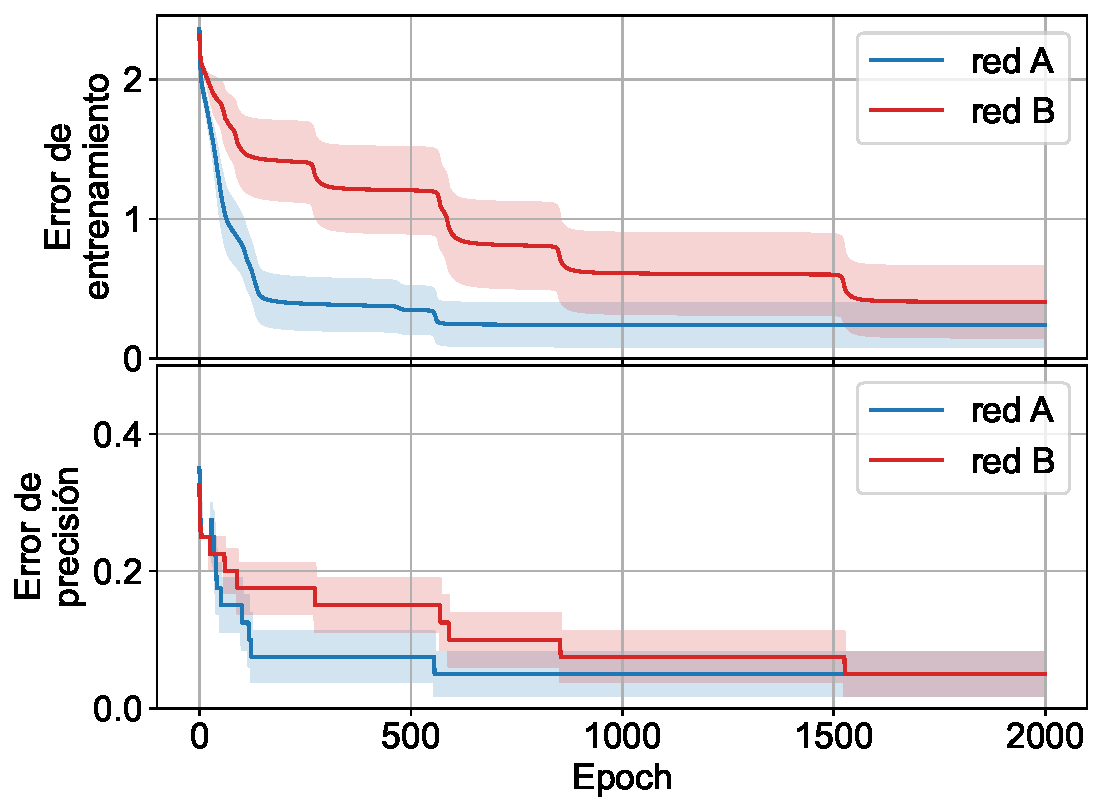
\includegraphics[clip=true,width=\columnwidth]{ej1_vs_epochs.pdf}
    \caption{Valor medio del a) error de entrenamiento y b) error de precisión en función de las epochs de entrenamiento para las arquitecturas A y B. El sombreado indica la desviación estándar del promedio.}
     \label{fig:ej1_error}
\end{figure}

\begin{figure}[h]
    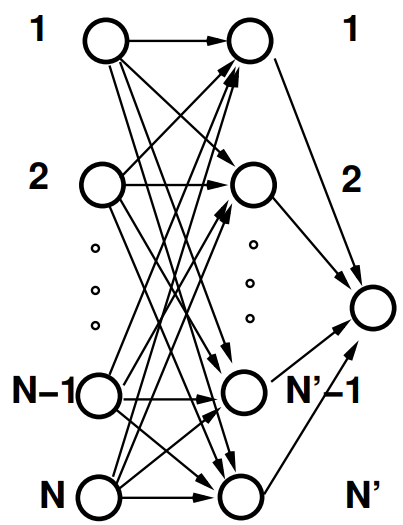
\includegraphics[clip=true,width=0.5\columnwidth]{ej2_arquitectura.png}
    \caption{Arquitectura utilizada para abordar el problema de paridad.}
     \label{fig:ej2_arquitectura}
\end{figure}


\begin{figure}
    {figure}[h]
        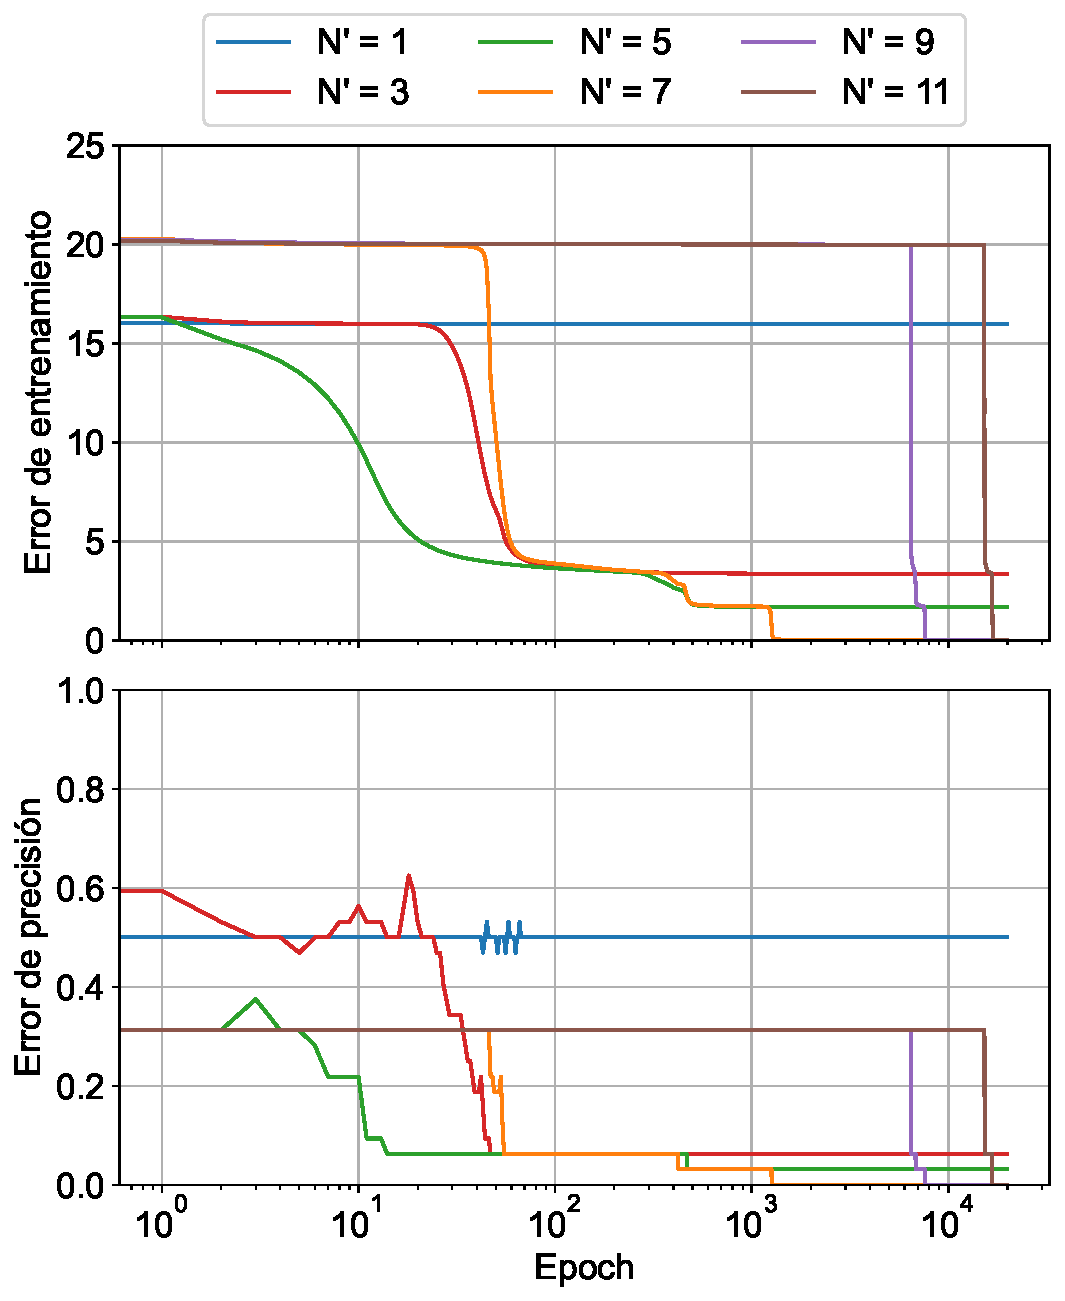
\includegraphics[clip=true,width=\columnwidth]{ej2_vs_epochs.pdf}
        \caption{a) Error de entrenamiento y b) error de precisión en función de las epochs de entrenamiento, variando el número de neuronas N’ en la capa oculta.}
         \label{fig:ej2_error}
\end{figure}
    
    

\begin{figure}[h]
    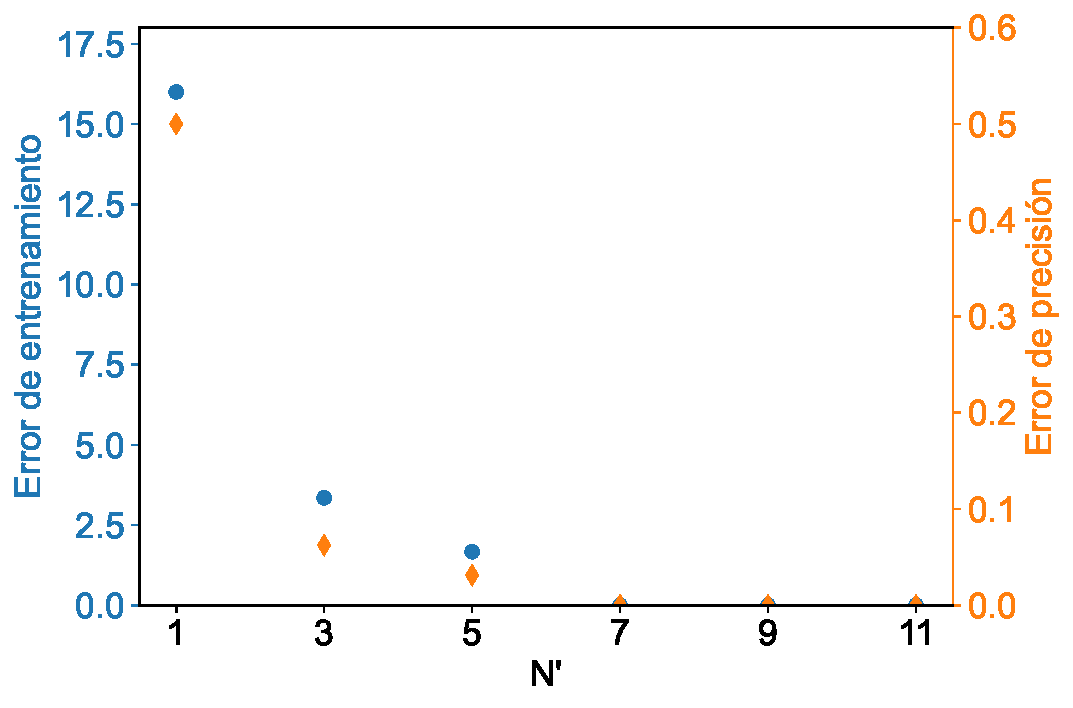
\includegraphics[clip=true,width=\columnwidth]{ej2_vs_N_prima.pdf}
    \caption{Error de entrenamiento y error de precisión final en función del número de neuronas N' en la capa oculta.}
        \label{fig:ej2_error_vs_Nprima}
\end{figure}

\begin{figure}[h]
    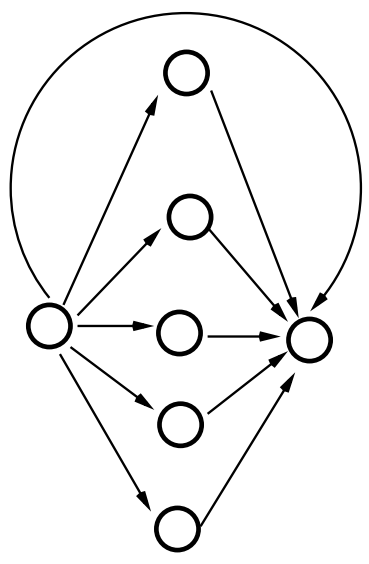
\includegraphics[clip=true,width=0.55\columnwidth]{ej3_arquitectura.png}
    \caption{Arquitectura adoptada para el aprendizaje del mapeo logístico.}
        \label{fig:ej3_arquitectura}
\end{figure}


\begin{figure}[h]
    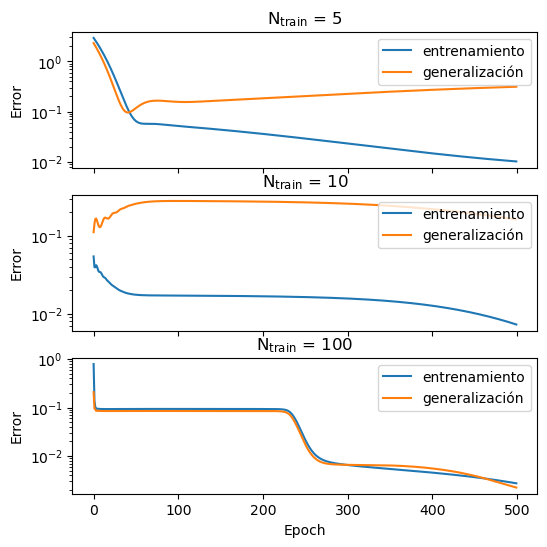
\includegraphics[clip=true,width=\columnwidth]{ej3_vs_epochs.png}
    \caption{Error de entrenamiento y error de precisión en función de las epochs de entrenamiento, para distintas cantidades de ejemplos \(N_{train}\) en los datos de entrenamiento.}
        \label{fig:ej3_error}
\end{figure}


El aprendizaje fue ejecutado mediante el algoritmo de retropropagación de errores (back-propagation), con pesos inicializados aleatoriamente con un valor máximo de 0.1 y un learning rate establecido en 0.1. La función de costo empleada fue el error cuadrático medio (MSE) y se utilizó $f(x) = tanh(x)$ como función de transferencia. Los datos de entrenamiento engloban todas las posibles combinaciones de entradas y salidas. Mientras que los datos de test corresponden al mismo conjunto de datos de entrenamiento.

En la Figura \ref{fig:ej1_error} se grafican los valores medios del error de entrenamiento y de precisión en función de las epochs para ambas arquitecturas, promediados sobre 10 condiciones iniciales de los pesos. En ambas arquitecturas, se evidencia una disminución de los errores a lo largo del tiempo, sin alcanzar un error nulo, posiblemente debido a que algunas redes se estabilizan en mínimos locales. De forma comparativa, la arquitectura A demuestra una velocidad de aprendizaje superior a la B.


Además, se observó cualitativamente que la velocidad de convergencia es influenciada por el valor máximo posible en la inicialización de los pesos y por el learning rate, existiendo configuraciones de ambos parámetros en las cuales el error no converge.

\section*{Ejercicio 2}



Se abordó la resolución del problema de paridad, extendiendo la lógica del XOR a N entradas. La arquitectura utilizada se muestra en la figura \ref{fig:ej2_arquitectura}, habiendo N' neuronas en la capa oculta y añadiendo una entrada adicional para simular el bias. El entrenamiento se llevó a cabo a través del algoritmo de retropropagación de errores, manteniendo la función de transferencia y la inicialización de los pesos idénticas al ejercicio previo y un learning rate de 0.05. Se establecieron N = 5 y N' = 1, 3, 5, 7, 9 y 11. Al igual que antes, los datos de entrenamiento engloban todas las posibles combinaciones de entradas y salidas. Mientras que los datos de test corresponden al mismo conjunto de datos de entrenamiento.


En la figura \ref{fig:ej2_error} se grafica el error de entrenamiento y de precisión en función de las epochs, explorando los diversos valores de N'.

Se observa que para N' = 1 el método converge pero con un gran error. Para N' = 3, la convergencia es más gradual hacia un error menor que el anterior pero distinto de cero. Con incrementos en N', la tendencia persiste: la convergencia es más lenta pero converge hacia errores progresivamente menores. Cuando N’ > 5, el error se anula pasado cierto número de epochs. Este fenómeno es evidenciado de forma más clara en la figura \ref{fig:ej2_error_vs_Nprima}, donde se grafica el error final en función de N'. Se observa que el error decae con el aumento de N', directamente relacionado con la complejidad de la red.



\section*{Ejercicio 3}

Se procedió al aprendizaje del mapeo logístico utilizando el método de retropropagación de errores, con la arquitectura representada en la figura \ref{fig:ej3_arquitectura} y añadiendo una entrada adicional para simular el bias. Se estableció un learning rate de 0.01 y, para las capas ocultas, se implementó la función de transferencia g(x) = 1/(1 + exp(-x)), mientras que la neurona de salida adoptó una función de activación lineal.

Se generaron los \(N_{train}\) datos de entrenamiento a través de la iteración del mapeo \(x(t + 1) = 4x(t)(1-x(t))\). De este modo, los datos corresponden a los pares {x(t), x(t+1)}. Además, se utilizaron 100 datos generados de manera análoga como ejemplos de prueba.



En la figura \ref{fig:ej3_error} se grafica el error de entrenamiento y el error de generalización, calculado sobre los datos de prueba, en función de las epochs. Para \(N_{train} = 5\) y 10, el comportamiento observado indica que, ante un número bajo de epochs, se está en condiciones de underfitting; luego, el error de generalización alcanza un mínimo y, posteriormente, aumenta, indicando una condición de overfitting. En cambio, para \(N_{train} = 100\), la gran cantidad de datos permite que ambos errores sean muy similares, sin llegar a presentar overfitting. Este comportamiento con variaciones en \(N_{train}\) se justifica en que el error de generalización tiende a disminuir con la cantidad de ejemplos.



\onecolumngrid

\section{Apéndice}
A continuación se desarrolla el código empleado durante este trabajo implementado en Python.




\begin{lstlisting}[language=Python]
  #Import libraries
  import matplotlib.pyplot as plt
  import numpy as np
  

\end{lstlisting}

\bibliography{Chehade_practica_4.bib}

\end{document}





